\documentclass{article}
\usepackage{tikz,pgfplots}

\pgfplotsset{compat=1.10}
\usepgfplotslibrary{fillbetween}

\begin{document}

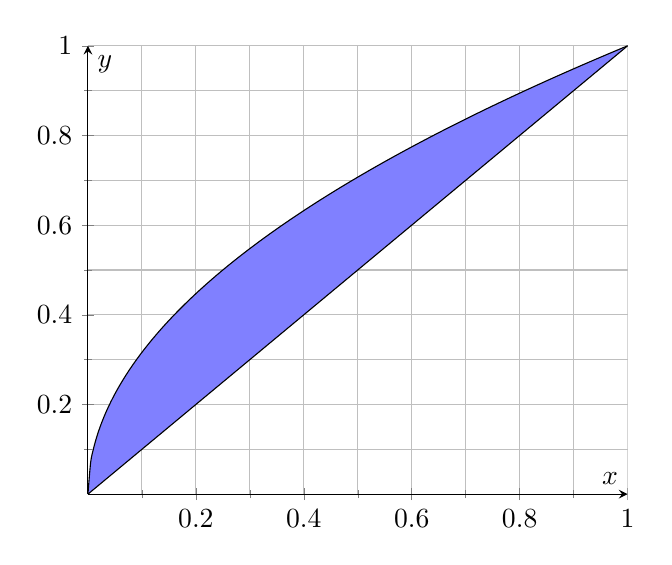
\begin{tikzpicture}
\begin{axis}[%set layers,
    axis lines = middle,
    smooth,
    no markers,
    xlabel = {$x$},
    ylabel = {$y$},
    minor tick num =1,
    grid=both,
    domain=0:2,]
        \addplot+[domain=0:1,samples=200,name path=A,black] {sqrt(x)};
        \addplot+[domain=0:1,name path=B,black] {x};
        \addplot[blue!50] fill between[of=A and B];
\end{axis}
\end{tikzpicture}

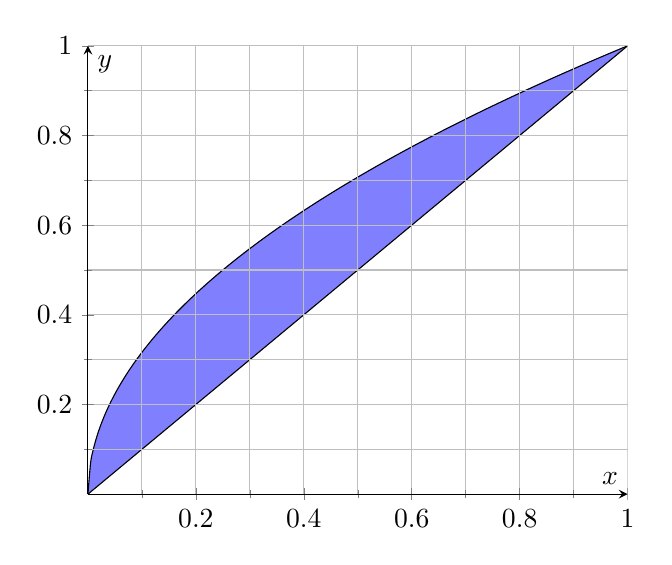
\begin{tikzpicture}
\begin{axis}[%set layers,
    axis lines = middle,
	axis on top,
    smooth,
    no markers,
    xlabel = {$x$},
    ylabel = {$y$},
    minor tick num =1,
    grid=both,
    domain=0:2,]
        \addplot+[domain=0:1,samples=200,name path=A,black] {sqrt(x)};
        \addplot+[domain=0:1,name path=B,black] {x};
        \addplot[blue!50] fill between[of=A and B];
\end{axis}
\end{tikzpicture}
\end{document}
